% =====================================================================
% WitnessRAG: a proposta (versão enxuta, no estilo da metodologia do GAM)
% Compilar: latexmk -pdf witnessrag-proposta-pt.tex
% Pouca matemática: apenas o necessário para entender a lógica da proposta.
% Detalhes de implementação estão em witnessrag-metodo-pt.tex.
% =====================================================================
\documentclass[11pt]{article}
\usepackage[margin=2.5cm]{geometry}
\usepackage[T1]{fontenc}
\usepackage[utf8]{inputenc}
\usepackage[brazilian, provide=*]{babel}
\usepackage{amsmath,amssymb,amsthm}
\usepackage{booktabs}
\usepackage{enumitem}
\usepackage{xcolor}
\usepackage{tikz}
\usetikzlibrary{arrows.meta,positioning,fit,backgrounds,shapes.geometric,calc}
\usepackage[hidelinks]{hyperref}

\newtheorem{definicao}{Definição}[section]
\newcommand{\op}[1]{\textsf{#1}}

\title{\textbf{WitnessRAG}\\[3pt]
\large Memória sob demanda orientada a testemunhas para agentes de linguagem}
\author{}
\date{Desenho da proposta, versão enxuta}

\begin{document}
\maketitle

\begin{abstract}
A memória de um agente de linguagem precisa entregar, a cada pedido, um
contexto pequeno que contenha o que é necessário para responder. Propomos o
\textbf{WitnessRAG}, uma memória que segue o princípio de compilação
\emph{just-in-time} e organiza o trabalho em dois módulos: um
\textbf{memorizador}, que preserva o histórico completo e o representa como
páginas e como fatos, e um \textbf{pesquisador}, que, para cada pergunta,
planeja o que precisa ser encontrado e procura uma \emph{testemunha}, isto é,
um conjunto mínimo de fatos que demonstra a resposta. A suficiência da
evidência é verificada por uma junção lógica sobre a memória, e não por uma
nova chamada ao modelo. O resultado é um contexto que parte de uma
recuperação forte e muda apenas onde há prova, com custo de duas ou três
chamadas por pergunta.
\end{abstract}

% =====================================================================
\section{Metodologia}

\subsection{Definição}

Seguimos a definição de memória do GAM: um sistema de memória produz, a
partir da tarefa e do histórico, o contexto que maximiza o desempenho do
agente com o menor tamanho possível,
\[
c^\ast \leftarrow \op{Memory}(\text{tarefa},\ \text{histórico}).
\]
No nosso cenário, o histórico é uma sequência de sessões
$H=(s_1,\dots,s_T)$, a tarefa é uma pergunta $q$ e o contexto é um conjunto de
$k$ páginas entregues a um leitor.

A pergunta central é \emph{o que} esse contexto deve conter. A nossa resposta
é: uma testemunha.

\begin{definicao}[Testemunha]
Seja $F$ o conjunto de fatos armazenados, $q$ uma pergunta e $a$ uma
resposta. Uma \emph{testemunha} de $a$ é um conjunto de fatos
$W\subseteq F$ que, em conjunto, demonstra que $a$ responde $q$, e do qual
nenhum fato pode ser retirado sem que a demonstração deixe de valer.
\end{definicao}

A propriedade que torna essa noção útil é simples: uma resposta pode ser
obtida de uma memória $S$ se, e somente se, pelo menos uma das suas
testemunhas está inteiramente contida em $S$,
\begin{equation}
a\in\mathrm{Ans}(q,S)\ \iff\ \exists\,W\ \text{testemunha de } a\ \text{com}\ W\subseteq S.
\label{eq:propriedade}
\end{equation}
Assim, preservar e recuperar respostas equivale a preservar e recuperar
testemunhas. Uma testemunha difere de um trecho \emph{relevante}: o segundo
elo de uma cadeia (``a Atlas fica em Recife'', para a pergunta ``onde fica o
empregador da Ana?'') pouco se parece com a pergunta, mas é indispensável
para respondê-la.

% =====================================================================
\subsection{WitnessRAG}

A arquitetura (Figura~\ref{fig:arquitetura}) tem dois módulos. O
\textbf{memorizador} trabalha uma vez, antes das perguntas, e mantém o
histórico completo em duas formas complementares: páginas de texto, para a
leitura, e fatos estruturados, para o raciocínio. O \textbf{pesquisador}
trabalha a cada pergunta: planeja, decide se vale a pena procurar uma prova,
compõe a testemunha quando possível e integra o resultado ao contexto. Os dois
módulos usam um modelo de linguagem com prompts específicos; a composição e a
verificação da testemunha são simbólicas.

\begin{figure}[t]
\centering
\resizebox{\textwidth}{!}{%
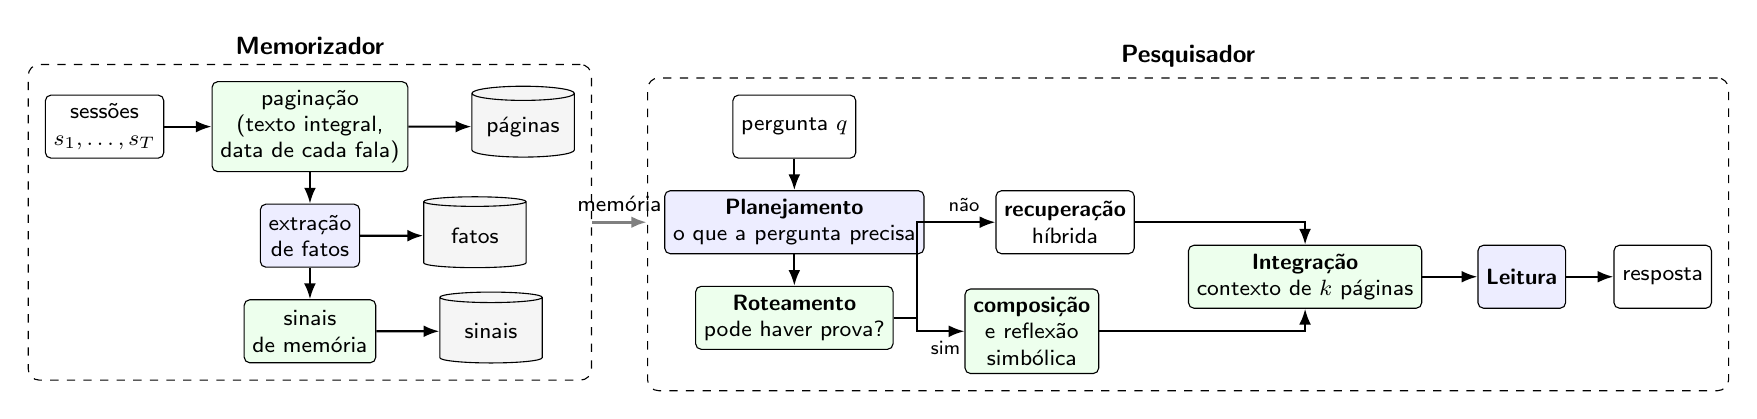
\begin{tikzpicture}[
  font=\sffamily\footnotesize, node distance=4mm and 6mm,
  box/.style={draw, rounded corners=2pt, align=center, minimum height=8mm,
              inner sep=3pt, fill=white},
  store/.style={draw, cylinder, shape border rotate=90, aspect=0.18,
                minimum height=9mm, minimum width=13mm, align=center,
                inner sep=1pt, fill=gray!8},
  llm/.style={box, fill=blue!7},
  sym/.style={box, fill=green!7},
  arr/.style={-{Latex[length=2mm]}, thick},
  grp/.style={draw, dashed, rounded corners=4pt, inner sep=6pt},
]
\node[box] (hist) {sessões\\$s_1,\dots,s_T$};
\node[sym, right=of hist] (page) {paginação\\(texto integral,\\data de cada fala)};
\node[llm, below=of page] (ie) {extração\\de fatos};
\node[sym, below=of ie] (sig) {sinais\\de memória};
\node[store, right=8mm of page] (P) {páginas};
\node[store, right=8mm of ie] (F) {fatos};
\node[store, right=8mm of sig] (S) {sinais};
\draw[arr] (hist) -- (page);
\draw[arr] (page) -- (P);
\draw[arr] (page) -- (ie);
\draw[arr] (ie) -- (F);
\draw[arr] (ie) -- (sig);
\draw[arr] (sig) -- (S);
\begin{scope}[on background layer]
  \node[grp, fit=(hist)(page)(ie)(sig)(P)(F)(S), label={[font=\sffamily\small\bfseries]above:Memorizador}] (mem) {};
\end{scope}
\node[box, right=20mm of P] (q) {pergunta $q$};
\node[llm, below=of q] (plan) {\textbf{Planejamento}\\o que a pergunta precisa};
\node[sym, below=of plan] (route) {\textbf{Roteamento}\\pode haver prova?};
\node[box, right=9mm of plan] (direct) {\textbf{recuperação}\\híbrida};
\node[sym, right=9mm of sig -| route.east, anchor=west] (compose) {\textbf{composição}\\e reflexão\\simbólica};
\coordinate (mid) at ($(direct.east)!0.5!(compose.east)$);
\node[sym, anchor=west] (integ) at ($(mid)+(9mm,0)$) {\textbf{Integração}\\contexto de $k$ páginas};
\node[llm, right=7mm of integ] (read) {\textbf{Leitura}};
\node[box, right=6mm of read] (ans) {resposta};
\draw[arr] (q) -- (plan);
\draw[arr] (plan) -- (route);
\draw[arr] (route.east) -- ++(3mm,0) |- node[pos=0.8, above, font=\sffamily\scriptsize]{não} (direct.west);
\draw[arr] (route.east) -- ++(3mm,0) |- node[pos=0.8, below, font=\sffamily\scriptsize]{sim} (compose.west);
\draw[arr] (direct.east) -| (integ.north);
\draw[arr] (compose.east) -| (integ.south);
\draw[arr] (integ) -- (read);
\draw[arr] (read) -- (ans);
\begin{scope}[on background layer]
  \node[grp, fit=(q)(plan)(route)(direct)(compose)(integ)(read)(ans), label={[font=\sffamily\small\bfseries]above:Pesquisador}] (res) {};
\end{scope}
\draw[arr, very thick, gray] (mem.east |- plan) -- node[above, black] {memória} (res.west |- plan);
\end{tikzpicture}}
\caption{Visão geral do WitnessRAG. O memorizador preserva o histórico como
páginas e fatos. O pesquisador planeja, decide se a pergunta admite prova,
compõe testemunhas quando admite e entrega um contexto pequeno ao leitor.
Azul: etapas com modelo de linguagem; verde: etapas simbólicas.}
\label{fig:arquitetura}
\end{figure}

% ---------------------------------------------------------------------
\subsubsection{Memorizador}

O memorizador processa o histórico sessão a sessão, com duas operações.

\paragraph{1. Paginação.} Cada sessão vira uma ou mais páginas que preservam o
texto integral. Cada página recebe um cabeçalho com a data da sessão, e cada
fala carrega o seu relógio de referência $\tau(u)$. Expressões relativas
(``ontem'', ``semana passada'') são normalizadas em relação a esse relógio e
anotadas ao lado da fala original:
\begin{equation}
\op{Memorizer.page}(s_i)\rightarrow p_i;\qquad \mathcal{P}.\op{append}(p_i).
\label{eq:page}
\end{equation}
Como no repositório de páginas do GAM, nada é resumido ou descartado.

\paragraph{2. Extração de fatos.} Cada página é convertida em fatos do tipo
(sujeito, relação, objeto, tempo), com o locutor resolvido e a página de
origem registrada. Menções diferentes da mesma entidade são unificadas, para
que a mesma coisa tenha sempre o mesmo nome:
\begin{equation}
\op{Memorizer.extract}(p_i)\rightarrow F_i;\qquad F\leftarrow F\cup F_i.
\label{eq:extract}
\end{equation}

A ligação entre cada fato e a sua página é o que permite, mais tarde, ir de
uma testemunha (fatos) de volta ao texto (páginas). O memorizador também
guarda alguns \emph{sinais de memória} simples, como a data de cada registro,
quantas vezes uma informação foi reafirmada e quão marcante emocionalmente é
cada fala, que o pesquisador pode usar depois.

% ---------------------------------------------------------------------
\subsubsection{Pesquisador}

O pesquisador atende a pergunta $q$ com as operações abaixo. Ele sempre parte
de uma recuperação híbrida (por significado e por palavras), cujas $k$
melhores páginas formam o contexto de base $B_k(q)$.

\paragraph{1. Planejamento.} Antes de buscar, o pesquisador descreve a
necessidade de informação num \emph{contrato de evidência}: que forma tem a
resposta (um nome, uma lista, uma data, um sim ou não), que raciocínio ela
exige (encontrar um fato, reunir vários, relacioná-los, calcular um tempo,
inferir algo não dito), se a evidência está num lugar ou em vários, que
entidades estão em foco, o que deve ser procurado e quais sinais de memória
são úteis:
\begin{equation}
\op{Researcher.plan}(q)\rightarrow\pi.
\label{eq:plan}
\end{equation}
O plano é escrito a partir da pergunta apenas. Não usa rótulos de tipo de
pergunta, respostas de referência ou qualquer anotação do benchmark: o
sistema entende sozinho o que está sendo pedido.

\paragraph{2. Roteamento.} O plano decide se a pergunta admite uma
testemunha. Isso acontece quando a resposta é uma entidade (ou um conjunto de
entidades) que decorre de vários fatos armazenados, reunidos ou relacionados
entre si. Perguntas que pedem um cálculo de tempo, uma inferência provável ou
um sim/não não têm testemunha a procurar e seguem com a recuperação híbrida:
\begin{equation}
\rho(\pi)\in\{\textsc{Compor},\ \textsc{Direta}\}.
\label{eq:route}
\end{equation}
O roteamento não classifica a pergunta por tipo: ele pergunta se pode existir
uma prova para ela.

\paragraph{3. Composição.} Na rota \textsc{Compor}, a pergunta é traduzida
numa consulta lógica: uma lista de condições que devem valer ao mesmo tempo,
com variáveis para o que ainda não se sabe. Por exemplo, ``onde fica o
empregador da Ana?'' vira ``existe $y$ tal que a Ana trabalha em $y$ e $y$
fica em $x$''. Em seguida, o pesquisador procura na memória de fatos
combinações que satisfaçam todas as condições com valores consistentes para
as variáveis:
\begin{equation}
\op{Researcher.compile}(q, F)\rightarrow Q;\qquad
\op{Researcher.join}(Q, F)\rightarrow\widehat{\mathcal{W}}.
\label{eq:compose}
\end{equation}
Cada combinação encontrada é uma testemunha candidata. Quando a pergunta pede
uma lista (``onde a Melanie já acampou?''), cada item da lista tem a sua
própria testemunha, e a resposta é o conjunto dos itens testemunhados.

\paragraph{4. Reflexão.} Em vez de perguntar a um modelo se a informação
reunida basta, o pesquisador examina o próprio resultado da junção. A prova é
aceita se existe testemunha e se ela é \emph{seletiva}: poucas respostas,
sem excesso de provas duplicadas, com casamentos confiáveis e cabendo no
espaço disponível. Se não for aceita, a falha é convertida em uma busca de
seguimento, formada pelas partes da consulta ou pelo ponto exato em que a
junção parou:
\begin{equation}
\op{Researcher.reflect}(\widehat{\mathcal{W}})\rightarrow y,\ r';\qquad
\text{se } y=\text{sim, devolve } \widehat{\mathcal{W}};\ \text{se } y=\text{não, busca } r'.
\label{eq:reflect}
\end{equation}

\paragraph{5. Integração.} O contexto final é o contexto de base com poucas
posições editadas: as páginas da testemunha, ou a página encontrada pela busca
de seguimento, ocupam as últimas posições, e as primeiras páginas da
recuperação híbrida são sempre preservadas:
\begin{equation}
\op{Researcher.integrate}\bigl(B_k(q),\ \widehat{\mathcal{W}},\ \Lambda\bigr)\rightarrow C(q).
\label{eq:integrate}
\end{equation}
O leitor recebe as \emph{páginas} de onde vieram os fatos, e não os fatos.
A testemunha decide o que mostrar; o texto original decide a resposta.

\paragraph{6. Leitura.} Um único leitor, o mesmo para todas as rotas, lê a
pergunta e o contexto, identifica a operação pedida e devolve uma resposta
curta: $\hat a\leftarrow\op{Reader}(q, C(q))$.

% ---------------------------------------------------------------------
\subsubsection{Lentes de memória}

Nem toda pergunta quer a memória mais parecida com ela: ``qual é o emprego
\emph{atual}'' quer a informação mais recente; ``onde morava \emph{na primavera
de 2021}'' quer registros daquela época; ``como ela \emph{se sentiu}'' quer as
falas mais marcantes. Inspirados na combinação de relevância, estabilidade
temporal e afetividade proposta em trabalhos anteriores do grupo, tratamos
esses sinais como \emph{lentes} que o próprio plano liga quando a pergunta
pede. Para uma página candidata $p$,
\begin{equation}
s(p\mid q,\pi)=R(p,q)\cdot\Bigl(1+\sum_{\ell\in\Lambda(\pi)}\Phi_\ell(p)\Bigr),
\label{eq:lens}
\end{equation}
em que $R$ é a relevância da recuperação e $\Phi_\ell$ é o sinal da lente
$\ell$: \textbf{temporal} (recência com decaimento, mais lento para
informações reafirmadas; proximidade a um período citado; ou prioridade ao
primeiro registro), \textbf{saliência} (intensidade emocional das falas da
pessoa em foco) e \textbf{confiança} (fatos confirmados por várias
extrações). A relevância multiplica: um registro irrelevante nunca é promovido
por ser recente ou emocional. As lentes apenas reordenam a cauda do contexto
e nunca removem páginas de uma testemunha.

% ---------------------------------------------------------------------
\subsubsection{Propriedades do desenho}

\paragraph{Intervenção limitada.} Toda decisão do pesquisador edita poucas
posições de um contexto que já é forte. Um erro de planejamento, de
compilação ou de junção custa, no pior caso, essas poucas posições.

\paragraph{Equivalência com um roteamento por rótulo.} Quando a rota escolhida
pelo plano coincide com a de um controlador que conhecesse o tipo da pergunta,
o contexto e a resposta são idênticos. Por isso, a diferença de desempenho
entre as duas versões é limitada pela fração de perguntas em que as rotas
discordam, que pode ser medida rodando apenas o planejador.

\paragraph{Custo.} Duas chamadas ao modelo por pergunta (planejamento e
leitura), ou três quando há composição (mais a compilação). Não há extração,
verificação ou replanejamento durante a resposta: a reflexão é simbólica.

\paragraph{Aprendizado ao longo do uso.} O desenho admite uma extensão
contínua: a participação de um fato em testemunhas de respostas confirmadas é
um sinal natural de utilidade, que pode reforçar esse fato nas buscas
seguintes, como a afetividade aprendida por reflexão. Nos experimentos, essa
atualização fica desligada, para que a resposta a uma pergunta não dependa das
perguntas anteriores.

% =====================================================================
\section{Configuração experimental}

\paragraph{Conjuntos de dados.} Seguimos o protocolo do GAM: LoCoMo
(perguntas de um salto, múltiplos saltos, temporais e de domínio aberto,
com as categorias usadas apenas para reportar resultados), HotpotQA com
memórias de 56K, 224K e 448K tokens, RULER a 128K tokens e NarrativeQA.

\paragraph{Linhas de base.} Métodos sem memória (LLM de contexto longo e RAG),
métodos baseados em grafo sobre a mesma base de fatos (GraphRAG, HippoRAG,
HippoRAG 2) e sistemas de memória (A-Mem, Mem0, MemoryOS, LightMem, GAM).

\paragraph{Perguntas de pesquisa.} (i) O planejamento sem rótulo preserva o
desempenho de um roteamento que conhece o tipo da pergunta? (ii) Como o
WitnessRAG se compara às linhas de base? (iii) Quanto contribuem o
roteamento, a composição e as lentes? (iv) Qual é o custo, e como o
desempenho varia com o número de posições que o pesquisador pode editar?

\paragraph{Detalhes.} Usamos GPT-4.1-mini e Qwen2.5-14B-Instruct como modelos
base, BGE-M3 para os embeddings, páginas de 2.048 tokens e um contexto de
$k=5$ páginas, com o mesmo leitor para todos os métodos.

\end{document}
